\chapter{Протоколы и стандарты локальных сетей}

\section{Протоколы и стандарты локальных сетей}

При организации взаимодействия узлов в локальных сетях основная роль отводится протоколу канального уровня.
Однако, для того, чтобы канальный уровень мог справиться с этой задачей, структура локальных сетей должна быть вполне определенной простой и регулярной.
Например, наиболее популярный протокол канального уровня - Ethernet - рассчитан на подключение всех узлов сети к общей шине, а протокол Token Ring рассчитан на соединение компьютеров в виде логического кольца.

\section{Особенности базовых технологий локальных сетей. Совместное использование линий связи конечными узлами}

Для удешевления аппаратных и программных решений разработчики первых локальных сетей \emph{остановились на совместном использовании кабелей всеми компьютерами сети в режиме разделения времени, то есть в режиме TDM}.
Наиболее явным образом режим совместного использования кабеля проявляется в сетях Ethernet, где общая шина физически представляет собой неделимый отрезок кабеля, общий для всех узлов сети.
Но и в сетях Token Ring и FDDI, где каждая соседняя пара компьютеров соединена, казалось бы, своими индивидуальными отрезками кабеля с концентратором, эти отрезки не могут использоваться компьютерами, которые непосредственно к ним подключены, в произвольный момент времени.
Эти отрезки образуют логическое кольцо, доступ к которому \emph{как к единому целому} может быть получен только по вполне определенному алгоритму, в котором участвуют все компьютеры сети.
Использование кольца как общего разделяемого ресурса упрощает алгоритмы передачи по нему кадров, так как в каждый конкретный момент времени кольцо используется только одним компьютером.

Использование \emph{разделяемых сред (shared media)} позволяет упростить логику работы сети.
Например, отпадает необходимость контроля переполнения узлов сети кадрами от многих станций, решивших одновременно обменяться информацией.
В глобальных сетях, где отрезки кабелей, соединяющих отдельные узлы, не рассматриваются как общий ресурс, такая необходимость возникает, и для решения этой проблемы в алгоритмы обмена информацией вводятся весьма сложные процедуры, предотвращающие переполнение каналов связи и узлов сети.

\section{Основные ограничения возможностей локальных сетей, вызванные применением простых конфигураций}

Использование в локальных сетях очень простых конфигураций (общая шина и кольцо) наряду с положительными имеют и негативные стороны, из которых наиболее неприятными являются \emph{ограничения по производительности и надежности}.
Наличие только одного пути передачи информации, разделяемого всеми узлами сети, в принципе ограничивало пропускную способность сети пропускной способностью этого пути (которая делилась в среднем на число компьютеров сети), а надежность сети - надежностью этого пути.
Поэтому по мере повышения популярности локальных сетей и расширения их сфер применения все больше стали применяться специальные коммуникационные устройства - коммутаторы и маршрутизаторы, - которые в значительной мере снимали ограничения единственной разделяемой среды передачи данных.
Базовые конфигурации в форме общей шины и кольца превратились в элементарные структуры локальных сетей, которые можно теперь соединять друг с другом более сложным образом, образуя параллельные основные или резервные пути между узлами.

Тем не менее, внутри базовых структур по-прежнему работают все те же протоколы разделяемых единственных сред передачи данных.
Это связано с тем, что хорошие скоростные и надежностные характеристики кабелей локальных сетей удовлетворяли в течение всех этих лет пользователей небольших компьютерных сетей, которые могли построить сеть без больших затрат только с помощью сетевых адаптеров и кабеля.
К тому же колоссальная инсталляционная база оборудования и программного обеспечения для протоколов Ethernet и Token Ring способствовала тому, что сложился следующий подход: в пределах небольших сегментов используются старые протоколы в их неизменном виде, а объединение таких сегментов в общую сеть происходит с помощью дополнительного и достаточно сложного оборудования.

\section{Разделямые сети, смешанные сети, сети с микросегментацией}

В последние несколько лет наметилось движение к отказу от разделяемых сред передачи данных в локальных сетях и \emph{переходу к применению активных коммутаторов, к которым конечные узлы присоединяются индивидуальными линиями связи}.
В чистом виде такой подход предлагается в технологии ATM (Asynchronous Transfer Mode), а в технологиях, носящих традиционные названия с приставкой switched (коммутируемый): switched Ethernet, switched Token Ring, switched FDDI. Обычно используется  смешанный подход, сочетающий разделяемые и индивидуальные среды передачи данных.
Чаще всего конечные узлы соединяются в небольшие разделяемые сегменты с помощью повторителей, а сегменты соединяются друг с другом с помощью индивидуальных коммутируемых связей.

Существует и достаточно заметная тенденция к использованию в традиционных технологиях так называемой \emph{микросегментации}, когда даже конечные узлы сразу соединяются с коммутатором индивидуальными каналами.
Такие сети получаются дороже разделяемых или смешанных, но производительность их выше.

\section{Полудуплексный и полнодуплексный режимы работы сетей}

При использовании коммутаторов у традиционных технологий появился новый режим работы - \emph{полнодуплексный (full duplex)}.
В разделяемом сегменте станции всегда работают в \emph{полудуплексном режиме (half duplex)},  так как в каждый момент времени сетевой адаптер станции либо передает свои данные, либо принимает чужие, но никогда не делает это одновременно.
Это справедливо для всех технологий локальных сетей, так как разделяемые среды  поддерживаются не только классическими технологиями локальных сетей Ethernet, Token Ring, FDDI, но и всеми новыми - Fast Ethernet, 100VG-AnyLAN, Gigabit Ethernet.

В полнодуплексном режиме сетевой адаптер может одновременно передавать свои данные в сеть и принимать из сети чужие данные.
Такой режим несложно обеспечивается при прямом соединении с мостом/коммутатором или маршрутизатором, так как вход и выход каждого порта такого устройства работают независимо друг от друга, каждый со своим буфером кадров.

\section{Структура стандартов IEEE 802.x}

В 1980 году в институте IEEE был организован комитет 802 по стандартизации локальных сетей, в результате работы которого было принято семейство стандартов IEEE 802.x, которые содержат рекомендации для проектирования нижних уровней локальных сетей.
Позже результаты его работы легли в основу комплекса международных стандартов ISO 8802-1...5.
Эти стандарты были созданы на основе очень распространенных фирменных стандартов сетей Ethernet, ArcNet и Token Ring.

Помимо IEEE в работе по стандартизации протоколов локальных сетей принимали участие и другие организации.
Так, для сетей, работающих на оптоволокне, американским институтом по стандартизации ANSI был разработан стандарт FDDI, обеспечивающий скорость передачи данных 100 Мб/с.
Работы по стандартизации протоколов ведутся также ассоциацией ECMA (European Computer Manufacturers Association), которой приняты стандарты ECMA-80, 81, 82 для локальной сети типа Ethernet и впоследствии стандарты ECMA-89, 90 по методу передачи маркера.

\section{Стандарты IEEE 802.x и уровни модели ВОС}

Стандарты семейства IEEE 802.x охватывают только два нижних уровня семиуровневой модели OSI - физический и канальный.
Это связано с тем, что именно эти уровни в наибольшей степени отражают специфику локальных сетей.
Старшие же уровни, начиная с сетевого, в значительной степени имеют общие черты, как для локальных, так и для глобальных сетей.

Специфика локальных сетей нашла также свое отражение в разделении канального уровня на два подуровня, которые часто называют также уровнями.
Канальный уровень (Data Link Layer) делится в локальных сетях на два подуровня:
\begin{itemize}
    \item логической передачи данных (Logical Link Control, LLC);
    \item управления доступом к среде (Media Access Control, MAC).
\end{itemize}

\section{Подуровни канального уровня стандартов локальных сетей}

\emph{Уровень MAC} появился из-за существования в локальных сетях разделяемой среды передачи данных.
Именно этот уровень обеспечивает корректное совместное использование общей среды, предоставляя ее в соответствии с определенным алгоритмом в распоряжение той или иной станции сети.
После того как доступ к среде получен, ею может пользоваться более высокий уровень - уровень LLC, организующий передачу логических единиц данных, кадров информации, с различным уровнем качества транспортных услуг.
В современных локальных сетях получили распространение несколько протоколов уровня MAC, реализующих различные алгоритмы доступа к разделяемой среде.
Эти протоколы полностью определяют специфику таких технологий как Ethernet, Fast Ethernet, Gigabit Ethernet, Token Ring, FDDI, 100VG-AnyLAN.

\emph{Уровень LLC} отвечает за передачу кадров данных между узлами с различной степенью надежности, а также реализует функции интерфейса с прилегающим к нему сетевым уровнем.
Именно через уровень LLC сетевой протокол запрашивает у канального уровня нужную ему транспортную операцию с нужным качеством.
 На уровне LLC существует несколько режимов работы, отличающихся наличием или отсутствием на этом уровне процедур восстановления кадров в случае их потери или искажения, то есть отличающихся качеством транспортных услуг этого уровня.

Протоколы уровней MAC и LLC взаимно независимы - каждый протокол MAC-уровня может применяться с любым типом протокола LLC-уровня, и наоборот.

\section{Структура стандартов IEEE 802}

Стандарты IEEE 802 имеют достаточно четкую структуру, появившуюся в результате большой работы, проведенной комитетом 802 по выделению в разных фирменных технологиях общих подходов и общих функций, а также согласованию стилей их описания.
В результате канальный уровень был разделен на два выше упомянутых подуровня.
Описание каждой технологии разделено на две части: описание уровня MAC и описание физического уровня.
Как видно из рисунка \ref{fig:ieee-802.x-standarts-structure}, практически у каждой технологии единственному протоколу уровня MAC соответствует несколько вариантов протоколов физического уровня (на рисунке в целях экономии места приведены только технологии Ethernet и Token Ring, но все сказанное справедливо также и для остальных технологий, таких как ARcNet, FDDI, 100VG-AnyLAN).

\section{Протокол LLC}

Над канальным уровнем всех технологий изображен общий для них протокол LLC, поддерживающий несколько режимов работы, независимо от выбора конкретной технологии.
Стандарт LLC курирует подкомитет 802.2.
Даже технологии, стандартизованные не в рамках комитета 802, ориентируются на использование протокола LLC, определенного стандартом 802.2, например протокол FDDI, стандартизованный ANSI.

\begin{figure}[!ht]
    \centering
    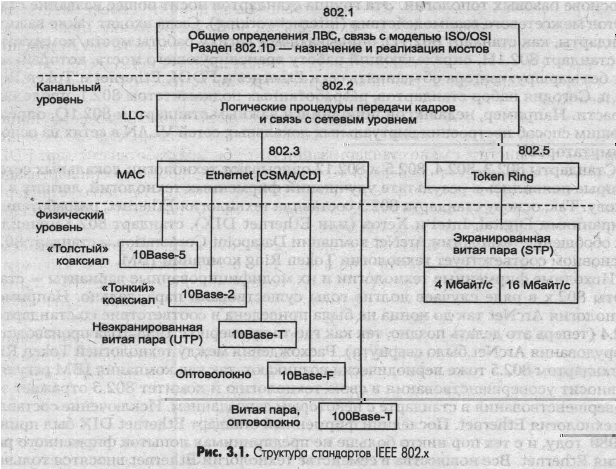
\includegraphics[width=0.9\textwidth]{ieee-802.x-standarts-structure}
    \caption{Структура стандартов IEEE 802.x}
    \label{fig:ieee-802.x-standarts-structure}
\end{figure}

\section{Протокол LLC уровня управления логическим каналом (802.2)}

Протокол LLC обеспечивает для технологий локальных сетей нужное качество услуг транспортной службы, передавая свои кадры либо дейтаграммным способом, либо с помощью процедур с установлением соединения и восстановлением кадров.
Протокол LLC занимает уровень между сетевыми протоколами и протоколами уровня MAC.
Протоколы сетевого уровня передают через межуровневый интерфейс данные для протокола LLC - свой пакет (например, пакет IP), адресную информацию об узле назначения, а также требования к качеству услуг, которое протокол LLC должен обеспечить.
Протокол LLC помещает пакет протокола верхнего уровня в свой кадр, который дополняется необходимыми служебными полями.
Далее через межуровневый интерфейс протокол LLC передает свой кадр вместе с адресной информацией об узле назначения соответствующему протоколу уровня MAC, который упаковывает кадр LLC в свой кадр (например, кадр Ethernet).

\section{Три типа процедур уровня LLC}

Первоначально в фирменных технологиях подуровень LLC не выделялся в самостоятельный подуровень, да и его функции растворялись в общих функциях протокола канального уровня.
Из-за больших различий в функциях  протоколов фирменных технологий, которые можно отнести к уровню LLC, на уровне LLC пришлось ввести три типа процедур.
Протокол сетевого уровня может обращаться к одной из этих процедур.

В соответствии со стандартом 802.2 уровень управления логическим каналом LLC предоставляет верхним уровням три типа процедур:
\begin{itemize}
    \item \emph{LLC1 - процедура без установления соединения и без подтверждения};
    \item \emph{LLC2 - процедура с установлением соединения и подтверждением};
    \item \emph{LLC3 - процедура без установления соединения, но с подтверждением}.
\end{itemize}

\emph{Процедура без установления соединения и без подтверждения LLC1} дает пользователю средства для передачи данных с минимумом издержек.
Это дейтаграммный режим.
Обычно, этот вид процедуры используется, когда такие функции, как восстановление данных после ошибок и упорядочивание данных выполняются протоколами вышележащих уровней, поэтому нет нужды дублировать их на уровне LLC.

\emph{Процедура с установлением соединений и с подтверждением LLC2} дает пользователю возможность установить логическое соединение перед началом передачи любого блока данных и, если это требуется, выполнить процедуры восстановления после ошибок и упорядочивание потока этих блоков в рамках установленного соединения.
Протокол LLC2 во многом аналогичен протоколам, которые применяются в глобальных сетях для обеспечения надежной передачи кадров на зашумленных линиях.
Протокол LLC2 работает в режиме скользящего окна.

В некоторых случаях (например, при использовании сетей в системах реального времени, управляющих промышленными объектами), когда временные издержки установления логического соединения перед отправкой данных неприемлемы, а подтверждение корректности приема переданных данных необходимо, базовая процедура без установления соединения и без подтверждения не подходит.
Для таких случаев предусмотрена дополнительная процедура, называемая процедурой без \emph{установления соединения, но с подтверждением LLC3}.

Использование одного из трех режимов работы уровня LLC зависит от стратегии разработчиков конкретного стека протоколов.
Например, в стеке TCP/IP уровень LLC всегда работает в режиме LLC1, выполняя простую работу извлечения из кадра и демультиплексирования пакетов различных протоколов – IP, ARP, RARP.
Аналогично используется уровень LLC стеком IPX/SPX.

\section{Структура кадров LLC}

\subsection{Типы кадров LLC}

По своему назначению все кадры уровня LLC (называемые в стандарте 802.
2 блоками данных - Protocol Data Unit, PDU) подразделяются на три типа - информационные, управляющие и ненумерованные:
\begin{itemize}
    \item
        \emph{Информационные кадры (Information)} предназначены для передачи информации в процедурах с установлением логического соединения LLC2 и должны обязательно содержать поле информации.
        В процессе передачи информационных блоков осуществляется их нумерация в режиме скользящего окна.

    \item
        \emph{Управляющие кадры (Supervisory)} предназначены для передачи команд и ответов в процедурах с установлением логического соединения LLC2, в том числе запросов на повторную передачу искаженных информационных блоков.

    \item
        \emph{Ненумерованные кадры (Unnumbered)} предназначены для передачи ненумерованных команд и ответов, выполняющих в процедурах без установления логического соединения передачу информации, идентификацию и тестирование LLC-уровня, а в процедурах с установлением логического соединения LLC2 - установление и разъединение логического соединения, а также информирование об ошибках.
\end{itemize}

Все типы кадров уровня LLC имеют единый формат.

\begin{table}[!ht]
    \centering
    \begin{tabular}{|m{0.12\textwidth}|m{0.17\textwidth}|m{0.15\textwidth}|m{0.15\textwidth}|m{0.1\textwidth}|m{0.12\textwidth}|}
        \hline
        Флаг (01111110) & Адрес точки входа сервиса назначения DSAP & Адрес точки входа сервиса источника SSAP & Управляющее поле Control & Данные Data & Флаг (01111110) \\ \hline
    \end{tabular}
\end{table}

Кадр LLC обрамляется двумя однобайтовыми полями «Флаг»,  имеющими значение 01111110.
Флаги используются на уровне MAC  для определения границ кадра LLC.
В соответствии с многоуровневой структурой протоколов стандартов IEEE 802, кадр LCC вкладывается в кадр уровня МАС: кадр Ethernet, Token Ring, FDDI и т.д.
При этом флаги кадра LLC отбрасываются.

Кадр LLC содержит поле данных и заголовок.

\subsection{Формат кадров LLC. Поле данных}

\emph{Поле данных кадра} LLC предназначено для передачи по сети пакетов протоколов вышележащих уровней – сетевых протоколов IP, IPX, AppleTalk, DECnet, в редких случаях - прикладных протоколов, когда те вкладывают свои сообщения непосредственно в кадры канального уровня.
Поле данных может отсутствовать в управляющих кадрах и некоторых ненумерованных кадрах.

\subsection{Формат кадров LLC. Заголовок}

Заголовок, в свою очередь, состоит из трех полей:
\begin{itemize}
    \item адрес точки входа службы назначения (Destination Service Access Point, DSAP);
    \item адрес точки входа службы источника (Source Service Access Point, SSAP);
    \item управляющее поле (Control).
\end{itemize}

\subsection{Формат кадров LLC. Заголовок – адресные поля}

\emph{Адресные поля DSAP и SSAP} занимают по 1 байту.
Они позволяют указать, какая служба верхнего уровня пересылает данные с помощью этого кадра.
Программному обеспечению узлов сети при получении кадров канального уровня необходимо распознать, какой протокол вложил свой пакет в поле данных поступившего кадра, для того, чтобы передать извлеченный из кадра пакет нужному протоколу для последующей обработки.
Для идентификации этих протоколов вводятся так называемые адреса точки входа службы (Service  Access Point, SAP).
Значения адресов SAP приписываются протоколам в соответствии со стандартом 802.2.
Например, для протокола IP значение SAP равно 0х6, для протокола NetBIOS - 0хF0.
Для одних служб определена только одна точка входа и, соответственно, только один SAP, а для других — несколько, когда адреса DSAP и SSAP совпадают.
Например, если в кадре LLC значения DSAP и SSAP содержат код протокола IРХ, то обмен кадрами осуществляется между двумя IРХ - модулями, выполняющимися в разных узлах.
Но в некоторых случаях в кадре LLC указываются различающиеся DSAP и SSAP.
Это возможно только в тех случаях, когда служба имеет несколько адресов SAP, что может быть использовано протоколом узла отправителя в специальных целях, например для уведомления узла получателя о переходе протокола-отправителя в некоторый специфический режим работы.
Этим свойством протокола LLC часто пользуется протокол NetBEUI.

\subsection{Формат кадров LLC. Заголовок – поле управления}
\emph{Поле управления (1 или 2 байта)} имеет сложную структуру при работе в режиме LLC2 и достаточно простую структуру при работе в режиме LLC1.

\begin{table}[!ht]
    \caption{Структура поля управления для кадров различного типа}
    \label{tab:control-sctructure}
    \centering
    \resizebox{\textwidth}{!}{%
        \begin{tabular}{|l|l|c|c|c|c|c|c|c|c|c|c|c|c|c|c|c|c|c|}
            \hline
                                       &                              & 1 & 2 & 3     & \multicolumn{2}{c|}{4}           & 5      & 6 & 7 & 8 & 9   & 10 & 11 & 12 & 13 & 14 & 15 & 16 \\ \hline
            \multirow{3}{*}{Тип кадра} & Информационный (Information) & 0 & \multicolumn{8}{c|}{N(S)}                                         & P/F & \multicolumn{7}{c|}{N(R)}        \\ \cline{2-19}
                                       & Управляющий(Supervisory)     & 1 & 0 & \multicolumn{2}{c|}{S} & \multicolumn{2}{c|}{-}   & - & - &   &     & \multicolumn{7}{c|}{N(R)}        \\ \cline{2-19}
                                       & Ненумерованный (Unnumbered)  & 1 & 1 & \multicolumn{2}{c|}{M} & \multicolumn{2}{c|}{P/F} & \multicolumn{11}{c|}{M}                            \\ \hline
        \end{tabular}%
    }
\end{table}

\section{Технология Ethernet (802.3)}
Ethernet - это самый распространенный на сегодняшний день стандарт локальных сетей.
Общее количество сетей, использующих в настоящее время Ethernet, оценивается в 5 миллионов, а количество компьютеров в них - в 50 миллионов.

В зависимости от типа физической среды стандарт IEEE 802.3 имеет различные модификации - 10Base-5, 10Base-2, 10Base-T, 10Base-FL, 10Base-FB.

Для передачи двоичной информации по кабелю для всех вариантов физического уровня технологии Ethernet, обеспечивающих пропускную способность 10 Мбит/с,  используется манчестерский код.

Все виды стандартов Ethernet используют один и тот же метод разделения среды передачи данных - метод CSMA/CD, который был впервые опробован во второй половине 60-х годов в радиосети Гавайского университета.

\subsection{Метод доступа CSMA/CD}
В сетях Ethernet используется метод доступа к среде передачи данных, называемый методом коллективного доступа с контролем несущей и обнаружением коллизий (carrier-sense-multiply-access with collision detection, CSMA/CD).

Этот метод используется исключительно в сетях с общей шиной все компьютеры которой имеют возможность одновременно (с учетом задержки распространения сигнала по физической среде) получить данные, которые любой из компьютеров начал передавать на общую шину.

Простота схемы подключения - это один из факторов, определивших успех стандарта Ethernet.
Говорят, что кабель, к которому подключены все станции, работает в режиме \emph{коллективного доступа (Multiply Access, MA)}.

\subsubsection{Этапы доступа к среде}
Все данные, передаваемые по сети, помещаются в кадры определенной структуры и снабжаются уникальным адресом станции назначения.

Чтобы получить возможность передавать кадр, станция должна убедиться, что \emph{разделяемая среда свободна}.
Это достигается прослушиванием основной гармоники сигнала, которая также называется несущей частотой (Carrier Sense, CS).
Признаком незанятости среды является отсутствие на ней несущей частоты, которая при манчестерском способе кодирования равна 5-10 МГц, в зависимости от последовательности единиц и нулей, передаваемых в данный момент.

\begin{figure}
    \centering
    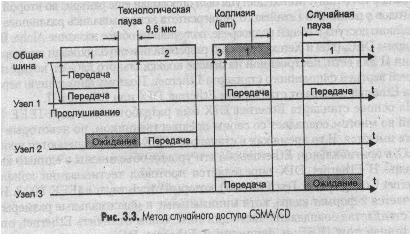
\includegraphics[width=0.7\textwidth]{CSMA-random-access}
    \caption{Метод случайного доступа CSMA/CD}
    \label{fig:CSMA-random-access}
\end{figure}

Если среда свободна, то узел имеет право начать передачу кадров.
Этот кадр изображен на рисунке первым.
Узел 1 обнаружил, что среда свободна, и начал передавать свой кадр.
Сигналы передатчика узла 1 распространяются в обе стороны, так что все узлы сети их получают.

Все станции, подключенные к кабелю, могут распознать факт передачи кадра, и та станция, которая узнает собственный адрес в заголовках кадра, записывает его содержимое в свой внутренний буфер, обрабатывает полученные данные и посылает по кабелю кадр-ответ.
Адрес станции-источника также включен в исходный кадр, поэтому станция-получатель знает, кому нужно послать ответ.

Узел 2 во время передачи кадра узлом 1 также пытался начать передачу своего кадра, однако обнаружил, что среда занята - на ней присутствует несущая частота, - поэтому узел 2 вынужден ждать, пока узел 1 не прекратит передачу кадра.

После окончания передачи кадра все узлы сети обязаны выдержать технологическую паузу (Inter Packet Gap) в $9.6 \text{~мкс}$.
Эта пауза, называемая также межкадровым интервалом, нужна для предотвращения монопольного захвата среды одной станцией.
После окончания технологической паузы узлы имеют  право начать передачу своего кадра, так как среда свободна.
Из-за задержек распространения сигнала по кабелю не все узлы строго одновременно фиксируют факт окончания передачи кадра узлом 1.

В приведенном примере узел 2 дождался окончания передачи кадра узлом 1,  сделал паузу 9,6 мкс и начал передачу своего кадра.

\subsubsection{Возникновение коллизии}
Механизм прослушивания среды и пауза между кадрами не гарантируют от возникновения такой ситуации, \emph{когда две или более станции одновременно решают, что среда свободна, и начинают передавать свои кадры}.
Говорят, что при этом происходит \emph{коллизия (collision)}, так как содержимое обоих кадров сталкивается на общем кабеле и происходит искажение информации.

\emph{Коллизия} - это нормальная ситуация в работе сетей Ethernet.
Для возникновения коллизии не обязательно, чтобы несколько станций начали передачу абсолютно одновременно, такая ситуация маловероятна.
Гораздо вероятней, что коллизия возникает из-за того, что один узел начинает передачу раньше другого, но до второго узла сигналы первого просто не успевают дойти к тому времени, когда второй узел решает начать передачу своего кадра.
То есть коллизии - это следствие распределенного характера сети.

Чтобы корректно обработать коллизию, все станции одновременно наблюдают за возникающими на кабеле сигналами.
Если передаваемые и наблюдаемые сигналы отличаются, то фиксируется обнаружение коллизии (collision detection, CD).
Для увеличения вероятности немедленного обнаружения коллизии всеми станциями сети, ситуация коллизии усиливается посылкой в сеть станциями, начавшими передачу своего кадра  специальной последовательности из 32 бит, называемой jam-последовательностью.

\begin{comment}

После обнаружения коллизии передающая станция прекращает передачу и ожидает в течение короткого случайного интервала времени.
Затем она снова делать попытку захвата среды и передачи кадра.
Случайная пауза выбирается по следующему алгоритму:
Пауза = L*(интервал отсрочки),
где интервал отсрочки равен 512 битовым интервалам (в технологии Ethernet принято все интервалы измерять в битовых интервалах, который обозначается как bt и соответствует времени между появлением двух последовательных бит данных на кабеле, для скорости 10 Мбит/с величина битового интервала равна 0,1 мкс или 100 нс).
L представляет собой целое число, выбранное с равной вероятностью из диапазона [0,2N], где N – номер повторной попытки передачи данного кадра: 1,2, …10.

   После 10-й попытки интервал, из которого выбирается пауза, не увеличивается.
Таким образом, случайная пауза может принимать значения от 0 до 52,4 мс.

   Если 16 последовательных попыток передачи кадра вызывают коллизию, то передатчик должен прекратить попытки и отбросить этот кадр.

Из описания метода доступа видно, что он носит вероятностный характер, и вероятность успешного получения в свое распоряжение общей среды зависит от загруженности сети.
При значительной интенсивности коллизий полезная пропускная способность сети Ethernet резко падает, так как сеть почти постоянно занята повторными попытками передачи кадров.
Для уменьшения интенсивности возникновения коллизий нужно либо уменьшить трафик, сократив, например, количество узлов в сегменте и заменив приложения, либо повысить скорость протокола.

Следует отметить, что метод доступа CSMA/CD вообще не гарантирует станции, что она когда-либо сможет получить доступ к среде.
Этот недостаток метода случайного доступа - плата  за его чрезвычайную простоту, которая сделала технологию Ethernet самой недорогой.
Другие методы доступа - маркерный доступ сети Token Ring и FDDI, метод Demand Priority сетей 100VG-AnyLAN - свободны от этого недостатка.

Время двойного оборота и распознавание коллизий.

Четкое распознавание коллизий всеми станциями сети является необходимым условием корректной работы сети Ethernet.
Если какая-либо передающая станция не распознает коллизию и решит, что кадр данных ею передан верно, то этот кадр данных будет отбракован принимающей станцией (скорее всего из-за несовпадения контрольной суммы).
Искаженная информация будет повторно передана каким-либо протоколом верхнего уровня, например, транспортным или прикладным, работающим с установлением соединения.
Но повторная передача сообщения протоколами верхних уровней произойдет через гораздо более длительный интервал времени (иногда даже через несколько  секунд) по сравнению с микросекундными интервалами, которыми оперирует протокол Ethernet, что приведет к заметному снижению полезной пропускной способности данной сети.

Для надежного распознавания коллизий должно выполняться следующее соотношение:  Tmin ≥PDV, где Tmin – время передачи кадра минимальной длины, а PDV – время, за которое сигнал коллизии успевает распространиться между двумя самыми взаимно удаленными узлами сети.
Так как в худшем случае сигнал должен пройти дважды этот путь (в одну сторону проходит неискаженный сигнал, а на обратном пути распространяется уже искаженный коллизией сигнал), то это время называется временем двойного оборота (Path Delay Value, PDV).

При выполнении этого условия передающая станция должна успевать обнаружить коллизию, которою вызвал переданный ее кадр, еще до того, как она закончит передачу этого кадра.
Очевидно, что выполнение этого условия зависит, с одной стороны, от длины минимального кадра и пропускной способности сети, а с другой стороны, от длины кабельной системы сети и скорости распространения сигнала в кабеле (для разных типов кабелей эта скорость несколько отличается).

В таблице приведены значения основных параметров процедуры передачи кадра стандарта 802.
3, которые не зависят от реализации физической среды.
Важно отметить, что каждый вариант физической среды технологии Ethernet добавляет к этим ограничениям  свои, часто более строгие ограничения, которые  также должны выполняться и которые будут ниже.

Таблица
Параметры уровня МАС Ethernet
Битовая скорость
10 Мбит/c
Интервал отсрочки
512 битовых интервалов
Межкадровый интервал
9.
6 мкс
Максимальное число попыток передачи
16
Максимальное число возрастания диапазона паузы
10
Длина jam-последовательности
32 бита
Максимальная длина кадра (без преамбулы)
1518 байтов
Минимальная длина кадра (без преамбулы)
64 байта (512 бит)
Длина преамбулы
64 бита
Минимальная длина случайной паузы после коллизии
0 битовых интервалов
Максимальная длина случайной паузы после коллизии
524 000 бит.
интервалов
Максимальное расстояние между станциями сети
2500 м
Максимальное число станций в сети
1024


Форматы кадров технологии Ethernet
По стандартам IEEE в сети Ethernet может использоваться только единственный вариант кадра канального уровня, образованный комбинацией заголовков МАС (стандарт 802.
3) и LLC (стандарт 802.
2) подуровней.

Тем не менее, на практике в сетях Ethernet на канальном уровне используются заголовки 4-х типов.
Основные отличия трех других заголовков связаны с тем, что до принятия стандартов IEEE 802 подуровень LLC не выделялся из общего канального протокола и, соответственно, заголовок LLC не применялся.

Консорциум трех фирм Digital, Intel и Xerox (DIX) в 1980 году представил на рассмотрение комитету 802.
3 свою версию стандарта Ethernet в качестве проекта международного стандарта.
Комитет 802.
3 принял стандарт, отличающийся в некоторых деталях от предложения DIX, причем отличия коснулись и формата кадра, что породило существование двух различных типов кадров Ethernet.

Еще один формат кадра появился в результате усилий  компании Novell по ускорению работы своего стека протоколов в сетях Ethernet.

И, наконец, четвертый формат кадра стал результатом деятельности комитета 802.
2 по приведению предыдущих форматов кадров к некоторому общему стандарту.

Один  и тот же тип кадра может иметь разные названия, поэтому ниже для каждого типа кадра приведено по несколько наиболее употребляемых названий:
Кадр 802.
3/LLC (кадр 802.
3/802.
2 или кадр Novell 802.
2)
Кадр Raw 802.
3 (или кадр Novell 802.
3)
Кадр Ethernet DIX (или кадр Ethernet II)
Кадр Ethernet SNAP
Форматы этих четырех типов кадров Ethernet приведены на рисунке.


Кадр 802.
3/LLC

6
6
2
1
1
1(2)
46-1497 (1498)
4
DA
SA
L
DSAP
SSAP
Control
Data
FCS






Заголовок LLC






Кадр Raw 802.
3 (или кадр Novell 802.
3)

6
6
2
46-1500
4
DA
SA
L
Data
FCS


Кадр Ethernet DIX (или кадр Ethernet II)

6
6
2
46-1500
4
DA
SA
L
Data
FCS


Кадр Ethernet SNAP

6
6
2
1
1
1(2)
3
2
46-1492
4
DA
SA
L
DSAP
SSAP
Control
OUI
T
Data
FCS






AA
AA
03
000000












Заголовок LLC
Заголовок SNAP






Кадр 802.
3/LLC
Заголовок кадра 802.
3/LLC является результатом объединения полей заголовков кадров MAC и LLC-уровней, определенных в стандартах IEEE  802.
3 и 802.
2, соответственно.


Кадр 802.
3/LLC

6
6
2
1
1
1(2)
46-1497 (1498)
4
DA
SA
L
DSAP
SSAP
Control
Data
FCS






Заголовок LLC






Стандарт 802.
3 определяет восемь полей заголовка:
Поле преамбулы состоит из семи байтов синхронизирующих данных, каждый из которых содержит одну и ту же последовательность битов - 10101010.
При манчестерском кодировании эта комбинация представляется в физической среде периодическим волновым сигналом с частотой 5 МГц.

Начальный ограничитель кадра (Start-of-frame-delimiter, SFD) состоит из одного байта с набором битов 10101011.
Появление этой комбинации  бит является указанием на то, что следующий байт – это первый байт заголовка кадра.
Преамбула и начальный ограничитель кадра обеспечивают побитовую и побайтовую синхронизацию (на рисунке не показаны).

Адрес назначения (Destination Address, DA) - может быть длиной 2 или 6 байт.
На практике всегда используются адреса из 6 байт.

Первый бит старшего байта адреса назначения является признаком того, является адрес  индивидуальным или групповым.
Если 0, то адрес является индивидуальным (unicast), а если 1, то это групповой адрес (multicast).
Групповой адрес сети может предназначаться всем узлам сети или же определенной группе узлов сети.
Если адрес состоит из всех единиц, то есть имеет шестнадцатеричное представление 0*FFFFFFFFFFFF, то он предназначен всем узлам сети и называется широковещательным адресом (broadcast).
В остальных случаях групповой адрес связан только с теми узлами, которые сконфигурированы (например, вручную) как члены группы, номер которой указан в групповом адресе.

Второй бит старшего байта адреса определяет способ назначения адреса – централизованный или локальный.
Если этот бит равен 0 (что бывает почти всегда в стандартной аппаратуре Ethernet), то адрес назначен централизованно, с помощью комитета IEEE.

Комитет IEEE распределяет между производителями оборудования так называемые организационно уникальные идентификаторы (Organizationally Unique Identifier, OUI).
Этот идентификатор помещается в 3 старших байтах адреса (например, идентификатор 000081 определяет компанию Bay Networks).

За уникальность младших 3-х байт адреса отвечает производитель оборудования.
Двадцать четыре бита, отводимые производителю для адресации интерфейсов его продукции, позволяют выпустить 16 миллионов интерфейсов под одним идентификатором организации.
Уникальность централизованно распределяемых адресов распространяется на все основные технологии локальных сетей – Ethernet, Token Ring, FDDI и т.
д.

Внимание:  В стандартах IEEE Ethernet младший бит байта изображается в самой левой позиции поля, а старший бит – в самой правой.
Это нестандартный способ отображения порядка бит в байте соответствует порядку  передачи бит в линию связи передатчиком Ethernet.

Адрес источника (Source Address, SA) - 2-х или 6-ти байтовое поле, содержащее адрес станции-отправителя кадра.
Первый бит всегда имеет значение 0.

Длина (Length, L).
Двухбайтовое поле длины определяет длину поля данных в кадре.

Поле данных (Data) может содержать от 0 до 1500 байт.
Но если длина поля меньше 46 байт, то используется следующее поле - поле заполнения, чтобы дополнить кадр до минимально допустимого значения в 46 байт.

Поле заполнения (Padding) состоит из такого количества байтов заполнителей, которое обеспечивает определенную минимальную длину поля данных (46 байт).
Это обеспечивает корректную работу механизма обнаружения коллизий.
Если длина поля данных достаточна, то поле заполнения в кадре не появляется.

Поле контрольной суммы (Frame Check Sequence, FCS) - 4 байта, содержащие значение, которое вычисляется по определенному алгоритму CRC-32.
После получения кадра рабочая станция выполняет собственное вычисление контрольной суммы для этого кадра, сравнивает полученное значение со значением поля контрольной суммы и, таким образом, определяет, не искажен ли полученный кадр.

Кадр 802.
3 является кадром MAС-подуровня, в соответствии со стандартом 802.
2 в его поле данных вкладывается кадр подуровня LLC с удаленными флагами начала и конца кадра.
Формат кадра LLC был описан выше.
Так как кадр LLC имеет заголовок длиной 3 (в режиме LLC1) или 4 байт (в режиме LLC2), то максимальный размер поля данных уменьшается до 1498 (1497) байт.

Кадр Raw 802.
3/Novell 802.
3
Кадр Raw 802.
3 или же кадр Novell 802.
3, представлен на рисунке, из которого видно, что это кадр MAC-подуровня стандарта 802.
3, но без вложенного кадра подуровня LLC.

Кадр Raw 802.
3 (или кадр Novell 802.
3)

6
6
2
46-1500
4
DA
SA
L
Data
FCS


Теперь, когда появилась необходимость идентификации протокола верхнего уровня, компания Novell стала использовать возможность инкапсуляции в кадр MAC-подуровня кадра LLC, то есть использовать стандартные кадры 802.
3/LLC.
Такой кадр компания обозначает теперь в своих операционных системах как кадр 802.
2, хотя он является комбинацией заголовков 802.
3 и 802.
2.

Кадр Ethernet DIX/ Ethernet II
Кадр Ethernet DIX, называемый также кадром Ethernet II, похож на кадр Raw 802.
3.
Однако 2-байтовое поле Длина (L) кадра Raw 802.
3 в кадре Ethernet DIX используется в качестве поля типа протокола.
Это поле, теперь получившее название Type (T) или EtherType,  предназначено для тех же целей, что и поля DSAP и SSAP кадра LLC - для указания типа протокола верхнего уровня, вложившего свой пакет в поле данных этого кадра.


Кадр Ethernet DIX (или кадр Ethernet II)

6
6
2
46-1500
4
DA
SA
L
Data
FCS


Кадр Ethernet SNAP
Для устранения разнобоя в кодировках типов протоколов, сообщения которых вложены в поле данных кадров Ethernet, комитетом 802.
2 была проведена работа по дальнейшей стандартизации кадров Ethernet.
В результате появился кадр Ethernet SNAP (SNAP - SubNetwork Access Protocol, протокол доступа к подсетям).

Кадр Ethernet SNAP

6
6
2
1
1
1(2)
3
2
46-1492
4
DA
SA
L
DSAP
SSAP
Control
OUI
T
Data
FCS






AA
AA
03
000000












Заголовок LLC
Заголовок SNAP





Кадр Ethernet SNAP представляет собой расширение кадра 802.
3/LLC путем введения дополнительного заголовка протокола SNAP, состоящего из двух полей: OUI и Type.
Поле Type состоит из 2-х байт и повторяет по формату и назначению поле Type кадра Ethernet II (то есть в нем используется те же значения кадров протоколов).
Поле OUI (Organizationally Unique Identifier)  определяет идентификатор организации, которая контролирует коды протоколов в поле Type.
С помощью заголовка SNAP достигнута совместимость с кодами протоколов в кадрах Ethernet II, а также создана универсальная схема кодирования протоколов.
Коды протоколов для технологий 802 контролирует IEEE, которая имеет OUI, равный 000000.
Если в будущем потребуются другие коды протоколов для какой-либо новой технологии, для этого достаточно указать другой идентификатор организации, назначающей эти коды, а старые значения кадров останутся в силе (в сочетании с другим идентификатором OUI).

Максимальная производительность сети Ethernet
Для коммуникационного оборудования наиболее тяжелым режимом является обработка кадров минимальной длины.
Это объясняется тем, что на обработку  каждого кадра мост, коммутатор или маршрутизатор тратит примерно одно и то же время, связанное с просмотром таблицы продвижения пакета, формированием нового кадра (для маршрутизатора) и т.
п.
А количество кадров минимальной длины, поступающих на устройство в единицу времени, естественно больше, чем количество кадров любой другой длины.

Максимальная производительность, определенная по кадрам минимальной длины
Используя параметры, приведенные в таблице, рассчитаем максимальную производительность сегмента Ethernet в таких единицах, как число переданных кадров (пакетов) минимальной длины в секунду.

Примечание:   При указании пропускной способности сети термины кадр и пакет обычно используются как синонимы.
Соответственно, аналогичными является и единицы измерения производительности  frames-per-second, fps и packets-per-second, pps.

Для расчета максимального количества кадров минимальной длины, проходящих по сегменту Ethernet, заметим, что размер кадра минимальной длины вместе с преамбулой составляет 72 байт или 576 бит, поэтому на его передачу затрачивается 57,5 мкс.
Прибавив межкадровый интервал в 9,6 мкс, получаем, что период следования минимальных пакетов равен 67,1 мкс.
Отсюда максимально возможная пропускная способность сегмента Ethernet в 14 880 кадр/с.



        57,5 мкс             9,6 мкс                      T=67,1 мкс



К расчету пропускной способности протокола Ethernet

Естественно, что наличие в сегменте нескольких узлов снижает эту величину за счет ожидания доступа к среде, а также за счет коллизий, приводящих к необходимости повторной передачи кадров.

Максимальная производительность, определенная по кадрам максимальной  длины
Кадры максимальной длины технологии Ethernet имеют поле длины 1500 байт, что вместе со служебной информацией дает 1518 байт, а с преамбулой составляет 1526 байт или 12 208 бит.
Максимально возможная пропускная способность сегмента Ethernet для кадров максимальной длины составляет 814 кадр/с.
Очевидно, что при работе с большими кадрами нагрузка на мосты, коммутаторы и маршрутизаторы довольно ощутимо снижается.

Максимальная полезная пропускная способность протокола
Теперь рассчитываем, какой максимальной полезной пропускной способностью в бит в секунду обладают сегменты Ethernet при использовании кадров разного размера.

Под полезной пропускной способностью протокола понимается скорость передачи пользовательских данных, которые переносятся полем данных кадра.
Эта пропускная способность всегда меньше номинальной битовой скорости протокола Ethernet за счет нескольких факторов:
Служебной информации кадров;
Межкадровых интервалов;
Ожидания доступа к среде.

Для кадров минимальной длины полезная пропускная способность равна:

Cn =14880*46*8 =5,48 Мбит/с.


Это намного меньше 10 Мбит/с, но следует учесть, что кадры минимальной длины используются в основном для передачи квитанций, так что к передаче собственно данных файлов эта скорость отношения не имеет.

Для кадров максимальной длины полезная пропускная способность равна:

Cn =813*1500*8 =9,76 Мбит/с,

что весьма близко к номинальной скорости протокола.

Еще раз подчеркиваем, что такой скорости можно достигнуть только в том случае, когда двум взаимодействующим узлам в сети Ethernet другие узлы не мешают, что бывает крайне редко.

При использовании кадров среднего размера с полем данных 512 байт пропускная способность сети составит 9,29 Мбит/с, что тоже достаточно близко к предельной пропускной способности в 10 Мбит/с.

Спецификации физической среды Ethernet
Исторически первые сети технологии Ethernet были созданы на коаксиальном кабеле диаметром 0,5 дюйма.
В дальнейшем были определены и другие спецификации физического уровня для стандарта Ethernet, позволяющие использовать различные среды передачи данных в качестве общей шины.
Метод доступа CSMA/CD и все временные параметры Ethernet остаются одними и теми же для любой спецификации физической среды.

Физические спецификации технологии Ethernet на сегодняшний день включают следующие среды передачи данных:
10Base-5 - коаксиальный кабель диаметром 0,5 дюйма, называемый "толстым" коаксиалом.
Имеет волновое сопротивление 50 Ом.
Максимальная длина сегмента - 500 метров (без повторителей).

10Base-2 - коаксиальный кабель диаметром 0,25 дюйма, называемый "тонким" коаксиалом.
Имеет волновое сопротивление 50 Ом.
Максимальная длина сегмента - 185 метров (без повторителей).

10Base-T - кабель на основе неэкранированной витой пары (Unshielded Twisted Pair, UTP).
Образует звездообразную топологию с концентратором.
Расстояние между концентратором и конечным узлом - не более 100 м.

10Base-F - оптоволоконный кабель.
Топология аналогична стандарту на витой паре.
Имеется несколько вариантов этой спецификации – FOIRL (расстояние до 1000 м), 10Base-FL (расстояние до 2000 м), 10Base-FB (расстояние до 2000 м).
\end{comment}
